\documentclass[runningheads]{llncs}

\usepackage{amssymb}
\usepackage{amsmath}
%% The amsthm package provides extended theorem environments

% \usepackage{amsthm}
% AM commented out because it clashes with proof, etc

%% The lineno packages adds line numbers. Start line numbering with
%% \begin{linenumbers}, end it with \end{linenumbers}. Or switch it on
%% for the whole article with \linenumbers.
\usepackage{lineno}

%% Use package enumitem to align enumeration and itemization
\usepackage{enumitem}
\usepackage{listings}
\usepackage{courier}           % for the courier font (optional)
\usepackage{multicol}          % for two equations side by side
\usepackage[justification=centering]{caption}
\usepackage[dvipsnames]{xcolor}
\usepackage{stmaryrd}
\usepackage{hyperref}
%\usepackage{cleveref}
\usepackage{hieroglf}
\usepackage{scalerel}
\usepackage{tikz}
\usepackage{pgfplots}
\usepackage[export]{adjustbox} % for subfigures
\usepackage{semantic}          % for mathlig


\hypersetup{ % play with these to change the look of hyperlinks
    colorlinks=true,
    linkcolor=black,
    filecolor=magenta,
    urlcolor=blue,
    citecolor=black
}

\newcommand{\coq}{\scalebox{.6}{\textpmhg{\Ha}}}
\newcommand{\p}[1]{\ensuremath{\mathsf{#1}}} % predicate font
\newcommand{\m}[1]{\ensuremath{\mathit{#1}}} % math font
\newcommand{\braces}[1]{\left\{\begin{array}{l@{}} #1 \end{array}\right\}}
\let\ramify\lightning
\newcommand{\sz}{\texttt{SIZE}}
\newcommand{\ifty}{\texttt{INF}}
\newcommand{\defeq}{\mathbin{\stackrel{\Delta}{=}}}
\usetikzlibrary{shadows}
\usetikzlibrary{arrows.meta, positioning, decorations.pathmorphing, fit, matrix}
\mathlig{/|}{\mathbin{\wedge}} % additive conjunction


% required by LNCS
\renewcommand\UrlFont{\color{blue}\rmfamily}

\colorlet{red}{red!80!black}
\colorlet{green}{green!50!black}

%% NEW COMMANDS =============================================

\lstdefinestyle{myStyle}{
%	language=Coq,
    keywords={Inductive,Require,Import,Definition,Fixpoint,match,with,end,let,in,fix},
	basicstyle=\normalfont\footnotesize\tt,
    keywordstyle=\color{green}, % Blue clashes with the cyan links. Change if you want.
	stepnumber=1,
	tabsize=2,
    numbers=none,
    numberstyle=\tiny,
    numbersep=5pt,
	showspaces=false,
    escapechar=`,
	showstringspaces=false
}
%basicstyle=\fontsize{10}{11}\selectfont\ttfamily,

\lstdefinestyle{myTinyStyle}{
%   language=Coq,
    basicstyle=\normalfont\fontsize{7.0}{7.3}\tt,
    keywordstyle=\color{green}, % Blue clashes with the cyan links. Change if you want.
    stepnumber=1,
    tabsize=2,
    numbers=none,
    numberstyle=\tiny,
    numbersep=5pt,
    showspaces=false,
    showstringspaces=false,
      language=C,
  morecomment=[l][{\color{OliveGreen}}]{//},
  sensitive=true,
  mathescape=true,
  showlines=true,
  escapechar=`,
  basicstyle=\footnotesize\ttfamily,
  keywordstyle=\color{blue}, numbers=left,
  numberstyle=\tiny, numbersep=5pt, boxpos=t
  }

\lstset{style=myTinyStyle}
\makeatletter
\newlength{\@mli}
\newcommand{\mli}[1]{%
  \settowidth{\@mli}{\lstinline/#1/}
  \hspace{-.5ex}\begin{minipage}[t]{\@mli}\lstinline/#1/\end{minipage}}
\makeatother
\newcommand{\li}[1]{\ifmmode\mbox{\mli{#1}}\else\mbox{\lstinline/#1/}\fi}

\newcommand\hide[1]{}

\newenvironment{centermath}
 {\begin{center}$\displaystyle}
 {$\end{center}}

\renewcommand{\note}[2][polish]{{\color{red} #2}{\marginpar{\tiny \color{blue} #1}}}
\renewcommand{\implies}{\Rightarrow}
\renewcommand{\iff}{\Leftrightarrow}

\title{A Machine-Checked C Implementation of Dijkstra's Shortest Path Algorithm}
\subtitle{(Short Paper)}
\titlerunning{A Machine-Checked C Implementation of Dijkstra's Shortest Path Algorithm}
%optional, please use if title is longer than one line

\begin{document}

\author{Anshuman Mohan$^{(\dagger)}$ \and Shengyi Wang$^{(\dagger)}$ \and Aquinas Hobor$^{(\dagger,\ddagger)}$}
\authorrunning{A. Mohan, S. Wang, A. Hobor}

%\author{Linh Tran \and Anshuman Mohan \and Aquinas Hobor}
%\authorrunning{L. Tran, A. Mohan, A. Hobor}
% First names are abbreviated in the running head.
% If there are more than two authors, 'et al.' is used.
%
\institute{($\dagger$) School of Computing and ($\ddagger$) Yale-NUS College, National University of Singapore}
% \\
% \email{\{hobor\}@comp.nus.edu.sg}}


\maketitle
%\begin{frontmatter}

%% Title, authors and addresses

%% use the tnoteref command within \title for footnotes;
%% use the tnotetext command for theassociated footnote;
%% use the fnref command within \author or \address for footnotes;
%% use the fntext command for theassociated footnote;
%% use the corref command within \author for corresponding author footnotes;
%% use the cortext command for theassociated footnote;
%% use the ead command for the email address,
%% and the form \ead[url] for the home page:

%% \tnotetext[label1]{}
%% \author{Name\corref{cor1}\fnref{label2}}
%% \ead{email address}
%% \ead[url]{home page}
%% \fntext[label2]{}
%% \cortext[cor1]{}
%% \address{Address\fnref{label3}}
%% \fntext[label3]{}

%% use optional labels to link authors explicitly to addresses:
%% \author[label1,label2]{}
%% \address[label1]{}
%% \address[label2]{}

%\author{}

%\address{}


\begin{abstract}
\vspace{-2em}
We report on a machine-checked proof of correctness for
Dijkstra’s one-to-all shortest path algorithm.
Unlike previous work, we use classic textbook code written in C.
Our C code is executable and realistic but also has real-world complications.
% We prove full functional correctness, and not just program safety.
Case in point, we show that Dijkstra’s algorithm suffers from
overflow issues for some inputs.
The precise bound in the relevant precondition is
nontrivial: we show that the intuitive guess
fails, and provide a workable refinement.

\keywords{Dijkstra \and verification \and coq}
\end{abstract}

%\end{frontmatter}

%% \linenumbers

%% main text

\section{Introduction}
\label{sec:intro}
Dijkstra's eponymous shortest-path algorithm~\cite{Dijk} finds
the cost-minimal paths from a distinguished \emph{source} vertex
source to all reachable vertices in a finite directed graph.

The algorithm is classic and ubiquitous, appearing widely in textbooks
and in real routing protocols. Further, the algorithm has been in
use for over $60$ years, suggesting, for all practical purposes,
that its safety and correctness have been verified by decades of application.

Recent efforts [cite Mizar, cite ACL2, cite Coq] have implemented the algorithm
in proof assistants and formally proved claims about its behavior.
However, because they operate entirely within idealized formal checkers,
these works inadvertently gloss over certain classes of issues
that routinely crop up in real-world settings.

In this paper we verify a~C~implementation of Dijkstra's
one-to-all shortest path algorithm. We implement
textbook~C~code [cite CLRS], import it into Coq [cite VST],
and state and prove a correctness claim in Coq [cite VST, cite RamifyCoq].
We expose a subtle overflow issue in the code, and address the issue
via a nontrivial refinement in the precondition of the algorithm.

The paper is organized as follows:
\vspace{-1em}
\begin{itemize}
    \item[\S\ref{sec:overview}] We briefly present and explain
    our~C~implementation of Dijkstra's algorithm.
    \item[\S\ref{sec:verification}] We present our specification
    and our most important loop invariant.
    \item[\S\ref{sec:overflow}] We explain the critical overflow issue
    in the code, and propose a fix by refinining the specification.
\end{itemize} 

\section{Verified Dijkstra in C}
\label{sec:overview}

Figure~\ref{fig:decorated} shows the code and proof
sketch of Dijkstra's algorithm.  Our code is implemented exactly
as suggested by CLRS~\cite{clrs} so we refer readers there for a
general discussion of the algorithm.
The adjacency-matrix-represented graph $\gamma$ of \texttt{SIZE} vertices
is passed as the parameter \texttt{graph} along with the source vertex \texttt{src}
and two allocated arrays \texttt{dist} and \texttt{prev}.
The details of the spatial predicates $\mathsf{array}(x,\vec{v})$, connecting an array pointer $x$ with its contents $\vec{v}$, and the internals of the priority
queue $\mathsf{PQ}$ are unexciting.  Our spatial graph predicate is more interesting in
that it nests arrays and connects the concrete memory values to an abstract mathematical
graph $\gamma$, which in turn exposes an interface in the language of graph theory
(vertices, edges, labels, etc.).

\begin{equation*}
\begin{split}
\m{list\_addr} ((\m{block}, \m{offset}), \m{index}) &\defeq
  (\m{block}, \m{offset} + (\m{index} \times \texttt{sizeof}(\texttt{int}) \times \texttt{SIZE})) \\
\p{list\_rep}(\gamma, \m{i}, \m{base\_ptr}) &\defeq \mathsf{array}(\mathsf{graph2matrix}(\gamma)[\m{i}], \m{list\_addr}(\m{base\_ptr}, \m{i})) \\
\vspace{1em}
\p{graph\_rep}(\gamma, \m{g\_addr}) &\defeq \underset{\m{v} \in \gamma}{\bigstar} \m{v}  \mapsto\p{list\_rep}(\gamma, \m{v}, \m{g\_addr})
\end{split}
\end{equation*}

In general these spatial representations are simple enough that they pose no special
challenge in the proof and so we will not focus on issues such as \emph{e.g.}~making
sure an array dereference is in bounds in our discussion below.

The key to the verification is the pure part of the loop
invariants on lines~\ref{code:whileinv} and~\ref{code:forinv}.  The \texttt{while} invariant $\m{dijk\_correct}(\gamma, \texttt{src}, \m{prev}, \m{dist}, \m{priq})$ has three parts:
\[
\begin{array}{l}
\forall \m{dst}.~\texttt{0} \le \m{dst} < \texttt{SIZE} -> \m{inv\_popped}(\gamma, \texttt{src}, \m{prev}, \m{dist}, \m{priq}, \m{dst}) /| \null \\
\hspace{11em}\m{inv\_unpopped}(\gamma, \texttt{src}, \m{prev}, \m{dist}, \m{priq}, \m{dst}) /| \null \\
\hspace{11em}\m{inv\_unseen}(\gamma, \m{prev}, \m{dist}, \m{priq}, \m{dst})
\end{array}
\]
A destination vertex $\m{dst}$ falls into one of three
categories:
\begin{enumerate}
\item $\m{inv\_popped}$: $\m{dst}$ has been fully processed, and has been
popped from the priority queue.
A globally optimal path from $\texttt{src}$
to $\m{dst}$ exists, the cost of this path is logged in
the \texttt{dist} array, and all the vertices visited by the path are also popped.
Further, the links of this path are logged in the \texttt{prev} array.
\item $\m{inv\_unpopped}$: $\m{dst}$ is reachable in
one hop from a ``\emph{mom}'' vertex, which is itself popped.
This route is locally optimal: we cannot
improve the cost by going via a \emph{different} popped vertex.
The \texttt{prev} array logs
\emph{mom} as the best-known way to reach $\m{dst}$, and the \texttt{dist}
array logs the cost of the path via \emph{mom} as the best-known cost.
\item $\m{inv\_unseen}$: no path is currently known from $\texttt{src}$ to $\m{dst}$.
\end{enumerate}
After popping the lowest-cost vertex in line~\ref{code:pop}, we reach the invariant of
the \texttt{for} loop $\m{dijk\_correct\_weak}(\gamma, \texttt{src}, \m{prev}, \m{dist}, \m{priq}, \texttt{i}, \texttt{u})$:
\[
\begin{array}{l}
\forall \m{dst}.~\texttt{0} \le \m{dst} < \texttt{SIZE} -> \m{inv\_popped}(\gamma, \m{src}, \m{prev}, \m{dist}, \m{priq}, \m{dst}) /| \null \\
\hspace{11em}\m{inv\_unseen}(\gamma, \m{prev}, \m{dist}, \m{priq}, \m{dst}) /| \null \\
\forall \m{dst}.~\texttt{0} \le \m{dst} < \texttt{i} -> \m{inv\_unpopped}(\gamma, \m{src}, \m{prev}, \m{dist}, \m{priq}, \m{dst}) /| \null \\
\forall \m{dst}.~\texttt{i} \le \m{dst} < \texttt{SIZE} -> \m{inv\_unpopped\_weak}(\gamma, \m{src}, \m{prev}, \m{dist}, \m{priq}, \m{dst}, \texttt{u})
\end{array}
\]
We now have four cases:
\begin{enumerate}
\item $\m{inv\_popped}$: $\m{dst}$ has been fully processed, and has been
popped from the priority queue.  For all popped vertices \emph{except for} \texttt{u}
this is trivial from $\m{dijk\_correct}$; for \texttt{u} itself we reach the heart of Dijkstra's correctness: the cost to the fringe vertex with minimum cost cannot be further improved.  The associated entailment is not trivial.
\item $\m{inv\_unseen}$: no path is currently known from $\texttt{src}$ to $\m{dst}$.  Trivially holds from $\m{dijk\_correct}$.
\item $\m{inv\_unpopped}$ (less than \texttt{i}): $\m{dst}$ is reachable in
one hop from a ``\emph{mom}'' vertex, which is itself popped.  Initially this is trivial since $\texttt{i}=0$ and we restore it as \texttt{i} climbs by updating costs when they can be improved in line~\ref{code:update}.
\item $\m{inv\_unpopped\_weak}$ (between than \texttt{i} and \texttt{SIZE}): ANSHUMAN
\end{enumerate}
The formal definitions for the above predicates, and the key subdefinitions upon which they rely, can be found in appendix~\ref{sec:apx}.

\hide{

While loop's invariant, which is stated on line
and explained further in Figure~\ref{fig:defns}.


This three-part invariant is trivially true before the while loop.
On line~\ref{code:pop}, the minimal vertex from the priority queue is popped,
thus breaking the invariant.

First, we must show that the minimal vertex $\m{u}$
obeys $\m{inv\_popped}$. \emph{i.e.}, show that the locally
optimal path to $\m{u}$ is, in fact, globally optimal.
This comes from blah blah blah

\newcommand{\s}{11}
\begin{figure}[htbp]
  \centering
  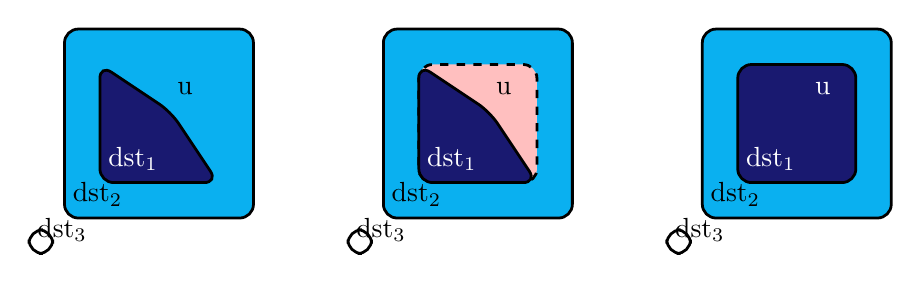
\begin{tikzpicture}[x=0.3cm, y=0.3cm,
      popped/.style={rounded corners=5pt, line width=1pt, draw, fill=MidnightBlue},
      fringe/.style={rounded corners=5pt, line width=1pt, draw, fill=ProcessBlue},
      popping/.style={rounded corners=5pt, line width=1pt, draw, dashed, fill=pink},
      unseen/.style={rounded corners=5pt, line width=1pt, draw}]
    \draw[unseen] (0,0) -- (\s,0) -- (\s,\s) -- (0,\s) -- cycle;
    \draw[fringe] (1.5,1.5) -- (9.5,1.5) -- (9.5,9.5) -- (1.5,9.5) -- cycle;
    \draw[popped] (3,3) -- (8,3) -- (6,6) -- (3,8) -- cycle;
    \node at (1.4,1) {dst$_3$};
    \node at (2.9,2.5) {dst$_2$};
    \node at (4.4,4) {\color{white}dst$_1$};
    \node at (6.6,7) {u};
    \tikzset{shift={(13.5,0)}}

    \draw[unseen] (0,0) -- (\s,0) -- (\s,\s) -- (0,\s) -- cycle;
    \draw[fringe] (1.5,1.5) -- (9.5,1.5) -- (9.5,9.5) -- (1.5,9.5) -- cycle;
    \draw[popping] (3,3) -- (8,3) -- (8,8) -- (3,8) -- cycle;
    \draw[popped] (3,3) -- (8,3) -- (6,6) -- (3,8) -- cycle;
    \node at (1.4,1) {dst$_3$};
    \node at (2.9,2.5) {dst$_2$};
    \node at (4.4,4) {\color{white}dst$_1$};
    \node at (6.6,7) {u};

    \tikzset{shift={(13.5,0)}}

    \draw[unseen] (0,0) -- (\s,0) -- (\s,\s) -- (0,\s) -- cycle;
    \draw[fringe] (1.5,1.5) -- (9.5,1.5) -- (9.5,9.5) -- (1.5,9.5) -- cycle;
    \draw[popped] (3,3) -- (8,3) -- (8,8) -- (3,8) -- cycle;
    \node at (1.4,1) {dst$_3$};
    \node at (2.9,2.5) {dst$_2$};
    \node at (4.4,4) {\color{white}dst$_1$};
    \node at (6.6,7) {\color{white}u};
  \end{tikzpicture}
  \caption{Popping $\m{u}$}
\end{figure}

Next, we must account for the ripple effect that popping
$\m{u}$ could have had on the other vertices.
In particular, it is possible that a vertex obeying $\m{inv\_unpopped}$ can
improve its cost via $\m{u}$, and that an unreachable vertex
obeying $\m{inv\_unseen}$ can now be reached via $\m{u}$.
The for loop repairs these breakages by
checking if a path via $\m{u}$ is an improvement for such vertices, and, if so,
edits both arrays and the priority queue as seen on line~\ref{code:update}.

The for loop's invariant is similar to that of the while loop---$\m{inv\_unseen}$
and $\m{inv\_popped}$ are preserved as-is, modulo the popping of
$\m{u}$ as discussed above. The key edit is in $\m{inv\_unpopped}$. blah blah blah

}



\begin{figure}[t]

\begin{lstlisting}[mathescape=true,showlines=true]
void dijkstra (int **g, int src, int *dist,
               int *prev, int size, int inf {
$\color{OliveGreen}//~\braces{\p{AdjMat}(\texttt{g},\gamma) *
\mathsf{array}(\texttt{dist}, \_) * \mathsf{array}(\texttt{prev}, \_)}$
 Item* temp = (Item*) mallocN(sizeof(Item));
 int* keys = mallocN (size * sizeof (int));
 PQ* pq = pq_make(size); int i, j, u, cost;
 for (i = 0; i < size; i++)
 { dist[i] = inf; prev[i] = inf; keys[i] = pq_push(pq,inf,i); } $\label{code:assigninf}$
 dist[src]= 0; prev[src]= src; pq_edit_priority(pq,keys[src],0);
 while (pq_size(pq) > 0) {
$\color{OliveGreen}//~\braces{{\color{red}\exists \m{dist}, \m{prev}, \m{popped}, \m{heap}}.~\p{AdjMat}(\texttt{g},\gamma) * {\color{red}\p{PQ}(\texttt{pq},\m{heap})} *
{\color{red}\mathsf{Item}(\texttt{temp}, \_)} * \null \\
\mathsf{array}(\texttt{dist},{\color{red}\m{dist}}) *
\mathsf{array}(\texttt{prev}, {\color{red}\m{prev}}) *
{\color{red}\mathsf{array}(\texttt{keys}, \m{keys}}) /| \null \\
{\color{red}\m{linked\_correctly}(\gamma, \m{heap}, \m{keys}, \m{dist}, \m{popped})} /| \null \\
{\color{red}\m{dijk\_correct}(\gamma,\texttt{src},\m{popped},\m{prev},\m{dist})}}$ $\label{code:whileinv}$
  pq_pop(pq, temp); u = temp->data; $\label{code:pop}$
  for (i = 0; i < size; i++) {
$\color{OliveGreen}//~\braces{{\color{red}\exists \m{dist'}, \m{prev'}, \m{heap'}}.~\p{AdjMat}(\texttt{g},\gamma) * \p{PQ}(\texttt{pq},{\color{red}\m{heap'}}) * \null \\
\mathsf{array}(\texttt{dist},\m{\color{red}dist'}) *
\mathsf{array}(\texttt{prev}, \m{\color{red}prev'}) *
\mathsf{array}(\texttt{keys}, \m{keys}) * \null \\
\mathsf{Item}(\texttt{temp}, \m{\color{red}(\texttt{keys[u]}, \texttt{dist[u]}, \texttt{u})}) /|
\m{\color{red}min(\texttt{dist[u]}, \m{heap'})} /| \null \\
{\m{linked\_correctly}(\gamma, \m{\color{red}heap'}, \m{keys}, \m{\color{red}dist'},
{\color{red}\m{popped} \uplus \{\texttt{u}\}})} /| \null \\
{\color{red}\m{dijk\_correct\_weak}({\color{OliveGreen}\gamma, \texttt{src}}, \m{popped} \uplus \{\texttt{u}\}, \m{prev'}, \m{dist'}, \texttt{i}, \texttt{u})}}$ $\label{code:forinv}$
   cost = getCell(g, u, i); $\label{code:cost}$
   if (cost < inf) {
    if (dist[i] > dist[u] + cost) { $\label{code:overflow}$
     dist[i] = dist[u] + cost; prev[i] = u; $\label{code:update1}$
     pq_edit_priority(pq, keys[i], dist[i]); $\label{code:update2}$
  }}}} $\color{OliveGreen}//~\braces{{\color{red}\exists \m{dist''}, \m{prev''}}.~\p{AdjMat}(\texttt{g},\gamma) * \p{PQ}(\texttt{pq},\m{\color{red}\emptyset}) * {\mathsf{Item}(\texttt{temp}, {\color{red}\_})} * \null \\
 \mathsf{array}(\texttt{dist},\m{\color{red}dist''}) *
 \mathsf{array}(\texttt{prev}, \m{\color{red}prev''}) *
 \mathsf{array}(\texttt{keys}, \m{keys}) /| \null \\
{\color{red}\forall \m{dst}.~0 \le \m{dst} < \texttt{size} -> \m{inv\_popped}}(\gamma, \m{src}, {\color{red}\m{\gamma.V}, \m{prev''}, \m{dist''}, \m{dst}})}$ $\label{code:end}$
 freeN (temp); pq_free (pq); freeN (keys); return; }
\end{lstlisting}
\vspace{-1em}
\caption{C code and proof sketch for Dijkstra's Algorithm.}
\vspace{-1em}
\label{fig:decorated}
\end{figure}



\hide{
$\color{OliveGreen}//~\braces{{\color{red}\exists \m{dist''}, \m{prev''},\m{heap''}}.~\p{AdjMat}(\texttt{g},\gamma) * \p{PQ}(\texttt{pq},\m{\color{red}heap''}) *
  \mathsf{array}(\texttt{dist},\m{\color{red}dist''}) * \null \\
  \mathsf{array}(\texttt{prev}, \m{\color{red}prev''}) *
  \mathsf{array}(\texttt{keys}, \m{keys}) *
  \mathsf{Item}(\texttt{temp}, \m{(\texttt{keys[u]}, \texttt{dist[u]}, \texttt{u})} /| \null \\
  \m{min(\texttt{dist[u]}, \m{heap'})} /|
  {\color{red}\m{heap''} = \m{heap'} [\texttt{keys[i]} \mapsto (\texttt{dist[i]},\texttt{i})]} /| \null \\
  {\m{\color{red}dijk\_correct}(\gamma, \texttt{src}, \m{popped'}, \m{\color{red}prev''}, \m{\color{red}dist''})}}$ $\label{code:caughtup}$
}



\section{I'm sorry Dave. I'm afraid I can't do that: Overflow}
\label{sec:overflow}
Dijkstra's algorithm clearly cannot work when a path
cost is greater than \texttt{INT\_MAX}.  A reasonable-looking restriction 
is to bound edge costs by 
$\left\lfloor\frac{\texttt{INT\_MAX}}{\texttt{size}-1}\right\rfloor$, since 
the longest optimal path has $\texttt{size}-1$ links and so the 
most expensive possible path costs no more than \texttt{INT\_MAX}.  
However, this has two flaws.  First, since we are writing real code in~C, 
rather than pseudocode in an idealized setting, we must reserve some 
concrete \texttt{int} value \texttt{inf} for ``infinity'', which has 
the special semantics that, if the best-known distance to a vertex~\m{x}
is \texttt{inf}, then~\m{x} is as-yet unreachable. 
A consequence of this is that reachable destination vertices cannot have a 
path cost of \texttt{inf}: if they did, this would be logged in the 
\m{dist} array and create an unpleasant ambiguity. 
Second, even though the best-known distances start at \texttt{inf} 
(see line~\ref{code:assigninf}) and only ever decrease from there, the code can 
overflow on lines~\ref{code:overflow}~and~\ref{code:update1}.

\begin{figure}[t]
\centering
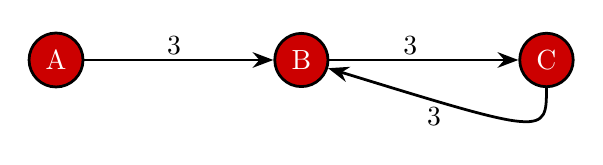
\begin{tikzpicture}[x=0.3cm, y=0.3cm,
  vert/.style={circle, line width=1pt, draw, fill=red}]
  \node[vert] (A) at (0,0) {\color{white}A};
  \node[vert] (B) [right = 8 of A] {\color{white}B};
  \node[vert] (C) [right = 8 of B] {\color{white}C};
  \draw [->,line width=1pt,arrows={-Stealth}] (A) -- (B);
  \draw [->,line width=1pt,arrows={-Stealth}] (B) -- (C);
  \draw [->,line width=1pt,arrows={-Stealth}] (C.south) .. controls ++(0, -2) .. (B);
  \node at (5,0.6) {3};
  \node at (15,0.6) {3};
  \node at (16,-2.4) {3};
\end{tikzpicture}
\caption{A graph that will result in overflow on a 3-bit machine.}
\label{fig:overflow}
\end{figure}

Consider applying Dijkstra's algorithm on a hypothetical 3-bit unsigned machine to 
the graph in figure~\ref{fig:overflow}.  The \texttt{size} of the graph is 3 nodes, and so the na\"ive edge-weight upper bound is $\left\lfloor\frac{\texttt{INT\_MAX}}{\texttt{size}-1}\right\rfloor = \left\lfloor\frac{7}{3-1}\right\rfloor = 3$, exactly as pictured in figure~\ref{fig:overflow}.  Indeed, a glance at the diagram is enough to tell that the true distance from the source~A~to vertices~B~and~C~are~3~and~6 respectively---both of which are representable with 3 bits, and so na\"ively all seems well.  %Unfortunately, Dijkstra's algorithm does not exactly work like that.  
Indeed, after processing vertices~A~and~B, 3~and~6~\emph{are} the costs reflected in the \m{dist} array for~B~and~C respectively---\emph{but unfortunately vertex~C~is still in the priority queue}.  After vertex~C~is popped on line~\ref{code:pop}, we fetch its neighbors in the \texttt{for} loop; vertex~B's cost of~3~is fetched on line~\ref{code:cost}.  On line~\ref{code:overflow} the currently optimal cost of~B~(3) is compared against the sum of the optimal cost of~C~(6) plus the just-retrieved cost of the edge from~C~to~B~(3).  Since $6+3$ overflows in 3-bit arithmetic, the comparison is not between~3~and~9 but in fact between~3~and~1!  Thus the code decides that a new cheaper path from~A~to~B~exists (in particular, A$\leadsto$B$\leadsto$C$\leadsto$B) and then trashes the \texttt{dist} and \texttt{prev} arrays on line~\ref{code:update1}.  %

Our code uses signed \texttt{int} rather than \texttt{unsigned int} so we have undefined behavior rather than defined-but-wrong behavior, but the essence of the overflow is identical.
Our solution is twofold.  First, we restrict the maximum edge cost to $\left\lfloor\frac{\texttt{INT\_MAX}}{\texttt{size+1}}\right\rfloor$, which in the 3-bit setting just described forces an edge cost of no more than~2.  Second, we require in the precondition that 
$\left\lfloor \frac{\texttt{INT\_MAX}}{\texttt{size}} \right\rfloor < \texttt{inf} \le \texttt{INT\_MAX} - \left\lfloor \frac{\texttt{INT\_MAX}}{\texttt{size}+1} \right\rfloor$, which in the 3-bit setting is 5.  Consider modifying figure~\ref{fig:overflow} to
have edge weights of~2~rather than~3.  After processing vertices~A~and~B, the distances to~B~and~C are no more than~2~and~4 respectively.  When we process vertex~C, the comparison on line~\ref{code:overflow} is thus between the previous best cost to~B~(2) and the candidate best cost to~B~via~C~(6); there is no overflow and the code behaves as advertised.



%% If you have bibdatabase file and want bibtex to generate the
%% bibitems, please use
%%
%\bibliographystyle{plainurl}% the mandatory bibstyle

\section{Future and Related Work; Conclusion}
\label{sec:conclusion}
\subsection{Related work}

We have already discussed work directly related to Dijkstra's (\S\ref{sec:relworkdijkstra}), Prim's (\S\ref{sec:relworkprim}), and Kruskal's (\S\ref{sec:relworkkruskal}) algorithms in detail, including work from both the algorithms and formal methods literature.  Summarizing briefly to the point of unreasonableness, our observations about Dijkstra's overflow and Prim's specification are novel, and existing formal proofs focus on code working within idealized environments rather than handling the real-world considerations that we do.  We have also already discussed the three formal developments we
build upon and extend: CompCert, VST, and CertiGraph (\S\ref{sec:stats}).  Our goal now is to discuss mechanized graph reasoning and verification more broadly.

\paragraph{Reasoning about mathematical graphs.}
There is a 30+ year history of mechanizing graph theory, beginning at least with Wong~\cite{wong1991} and Chou~\cite{chou1994formal} and continuing to the present day; Wang discusses many such efforts~\cite[\S3.3]{shengyi:thesis}.  The two abstract frameworks that seem closest to ours are those by Noschinski~\cite{Noschinski2015}; and by Lammich and Nipkow~\cite{DBLP:journals/afp/LammichN19}.  The latter is particularly related to our work, because they too start with a directed graph library and must extend it to handle undirected graphs so that they can verify Prim's algorithm.

\paragraph{More-automated verification.}
Broadly speaking, mechanized verification of software falls in a spectrum between more-automated-but-less-precise verifications and less-automated-but-more-precise verifications.  Although VST contains some automation, we fall within the latter camp.  In the former camp, landmark initial separation logic~\cite{reynolds2002separation} tools such as Smallfoot~\cite{berdine:smallfoot} have grown into Facebook's industrial-strength Infer~\cite{calcagno2015moving}.  Other notable relatively-automated separation logic-based tools include HIP/SLEEK~\cite{chin:hipsleek}, Bedrock~\cite{chlipala:bedrock}, and VerCors~\cite{DBLP:conf/fm/BlomH14}.  More-automated solutions that use techniques other than separation logic include Boogie~\cite{barnett2005boogie}, \textsc{Blast}~\cite{DBLP:journals/sttt/BeyerHJM07}, Dafny~\cite{leino10}, and KeY~\cite{DBLP:series/lncs/10001}.  In \S\ref{sec:relworkdijkstra} we discuss how some of these more-automated approaches have been applied to verify Dijkstra's algorithm. Petrank and Hawblitzel's Boogie-based verification of a garbage collector~\cite{gcexample2} gives another more-automated verification of a graph algorithm.

We are not confident that more-automated tools would be able to replicate our work easily.  We prove full functional correctness, whereas many more-automated tools prove only more limited properties.  Moreover, our full functional correctness results rely upon a meaningful amount of domain-specific knowledge about graphs, which automated tools usually lack.  Even if we restrict ourselves to more limited domains such as overflows, several more automated efforts did not uncover the overflow that we described in \S\ref{sec:relworkdijkstra}.  The proof that certain bounds on edge weights and \texttt{inf} suffice depends on an intimate understanding of Dijkstra's algorithm (in particular, that it explores one edge beyond the optimum paths); overall the problem seems challenging in highly-automated settings.  The more powerful specification we discover for Prim's algorithm in \S\ref{sec:primforest} is likewise not something a tool is likely to discover: human insight appears necessary, at least given the current state of machine learning techniques.

In contrast, several of the potential overflows in our binary heap might be uncovered by more-automated approaches, especially those related to the \texttt{PARENT} and \texttt{LEFT\_CHILD} macros from \S\ref{sec:heapinsertremove}.  Although the arithmetic involves both addition/subtraction and multiplication/division, we suspect a tool such as Z3~\cite{moura2008} could handle it. \hide{; the multiplication/division always has the constant \texttt{2u} for an operand.}  Moreover, a sufficiently-precise tool would probably spot the necessity of forcing the internal constants into \texttt{unsigned int}.  The issue of sound key generation described in~\S\ref{sec:modpri} might be a bit trickier.  On the one hand, \texttt{unsigned int} overflow is defined in~C, so real code sometimes relies upon it.  Accordingly, merely observing that the counter could overflow does not guarantee that the code is necessarily buggy.  On the other hand, some tools might flag it anyway out of caution (\emph{i.e.} right answer, wrong reason).

\paragraph{Less-automated verification.}
Although as discussed above some more-automated tools have been applied to verify graph algorithms, the problem domain is sufficiently complex that many of the verifications discussed in \S\ref{sec:relworkdijkstra}, \S\ref{sec:relworkprim}, and \S\ref{sec:relworkkruskal} use less-automated techniques.  Two basic approaches are popular.  The ``shallow embedding'' approach is to write the algorithm in the native language of a proof assistant.  The ``deep embedding'' approach is to write the algorithm in another language whose semantics has been precisely defined in the proof assistant.  VST uses a deep embedding, and so we do too; one of VST's more popular competitors in the deep embedding style is ``Iris Proof Mode''~\cite{DBLP:conf/popl/KrebbersTB17}.  In contrast, Lammich \emph{et al.} have produced a series of results verifying a variety of graph algorithms using a shallow embedding~(\emph{e.g.},~\cite{DBLP:conf/itp/Lammich14,DBLP:journals/afp/LammichN19,DBLP:journals/afp/HaslbeckLB19,DBLP:journals/jar/LammichS19,DBLP:conf/itp/LammichS16}).  From a bird's-eye view Lammich \emph{et al.}'s work is the most related to our results in this paper: they verify all three algorithms we do and are able to extract fully-executable code, even if sometimes their focus is a bit different, \emph{e.g.} on novel purely-functional data structures such as a  priority queue with \texttt{edit\_priority}.  %In particular, Lammich \emph{et al.} are able to ; others such as Guttmann provide only relational program descriptions and so probably cannot~\cite{DBLP:conf/ictac/Guttmann16,DBLP:journals/jlp/Guttmann18}.

Although not related to the main thrust of this paper, Lammich has verified Introsort~\cite{DBLP:conf/cade/Lammich20}, which includes a heapsort much like the one we present in \S\ref{sec:heapsort}.  He generates LLVM code, \emph{i.e.} uses a deep embedding.

%we note that Lammich has an ``approach B'' (deep embedding, in the sense that he generates LLVM code) verification of Introsort, which combines quicksort, heapsort, and insertion sort.

\paragraph{Pen-and-paper verification of graph algorithms.}

We use separation logic~\cite{reynolds2002separation} as our base framework.  Initial work on graph algorithms in separation logic was minimal; Bornat \emph{et al.} is an early example~\cite{bornat:aliasing04}.  Hobor and Villard developed the technique of ramification to verify graph algorithms~\cite{hobor:ramification}, using a particular ``star/wand'' pattern to express heap update.  Wang \emph{et al.} later integrated ramification into VST as the CertiGraph project we use~\cite{DBLP:journals/pacmpl/WangCMH19}.  Krishna \emph{et al.}~\cite{krishna2017go} have developed a flow algebraic framework to reason about local and global properties of \textit{flow graphs} in the program heap; their flow algebra is mainly used to tackle local reasoning of global graphs in program heaps.
Flow algebras should be compatible with existing separation logics; implementation and integration with the Iris project appears to be work in progress~\cite{DBLP:conf/esop/KrishnaSW20}.

Krishna \emph{et al.} are interested in concurrency~\cite{krishna2017go}; Raad \emph{et al.} provide another example of pen-and-paper reasoning about concurrent graph algorithms~\cite{DBLP:conf/aplas/RaadHVG16}.

\vspace*{-0.25em}

\subsection{Future work}

\vspace*{-0.25em}

We see several opportunities for decreasing the effort and/or increasing the automation in our approach.  At the level of Hoare tuples, we see opportunities for improved VST tactics to handle common cases we encounter in graph algorithms.  At the level of spatial predicates, we can continue to expand our library of graph constructions, for example for adjacency lists.  We also believe there are opportunities to increase modularity and automation at the interface between the spatial and the mathematical levels, \emph{e.g.} we sometimes compare~C~pointers to heap-represented graph
nodes for equality, and due to the nature of our representations this equality check will be
well-defined in~C~when the associated nodes are present in the mathematical graph, so this check should pass automatically.

We believe that more automation is possible at the level of mathematical graphs: for example reachability techniques based on regular expressions over matrices and related semirings~\cite{backhouse,DBLP:journals/jacm/Tarjan81a,dolan2013fun}.  We are also intrigued by the recent development of various specialized graph logics such as by Costa \emph{et al.}~\cite{costa:graphlogic} and hope that these kinds of techniques will allow us to simplify our reasoning.
The key advantage of having end-to-end machine-checked examples such as the ones we presented above is
that they guide the automation efforts by providing precise goals that are known to be strong
enough to verify real code.

\vspace*{-0.25em}
\subsection{Conclusion}
\vspace*{-0.25em}

We extend the CertiGraph library to handle undirected graphs and several flavours of graphs with edge labels, both at the pure and at the spatial levels.  We have verified the full functional correctness of the three classic graph algorithms of Dijkstra, Prim, and Kruskal.  We find nontrivial bounds on edge costs and infinity for Dijkstra and provide a novel specification for Prim.  We have verified a binary heap with Floyd's \texttt{heapify} and \texttt{edit\_priority}.
All of our code is in CompCert~C~and all of our proofs are machine-checked in Coq.

\paragraph{Acknowledgements.}  We thank Shengyi Wang for some help with understanding the CertiGraph implementation, as well as a useful initial discussion about understanding the program invariants of Dijkstra's algorithm.

%The existing library of CertiGraph verifications contains a treasure trove of \emph{precisely} what lemmas are needed to verify real graph code, which should help to guide the development of automated techniques.

%; and (D) improved modularity in our constructions and
%automation of common cases

% such as the adjacency-matrix representation used in this result, as well as associated lemmas;

%are interested in increasing the amount of automation in our approach.

%\paragraph{Verifying graph algorithms}

%mention Iris?

%Brotherston

%Automated graph work / future work

%\note{Being in pseudocode and , these works do not need to discuss the application of the algorithms on "strange", non-simple graph inputs. Our C implementation does account for such inputs to a small extent, such as the edge list containing multiple edges between two vertices in Kruskal's.}

%\paragraph{Other graph proof libraries.}

%\cite{DBLP:conf/esop/KrishnaSW20}

%, tackling similar issues to Wang et al ~\cite{DBLP:journals/pacmpl/WangCMH19}, but in this paper, local reasoning is not required.
%In a related vein, Paulin and Filli\^atre verified Floyd's algorithm in Coq~\cite{paulin}
%
%\subsection{Previous work} We have long been interested in
%the verification of graph-manipulating programs written in~C~.
%We fortified our techniques to handle realistic (CompCert~\cite{leroy:compcert})~C~to a machine-checked level of rigour~\cite{DBLP:journals/pacmpl/WangCMH19}.  Novel features of the present result include a previously-untried adjacency matrices spatial graph representation as well as non-trivial edge labels between graph nodes. % for the first time. %, used to represent cost. %; both are new for us.
%
%\subsection{Ongoing and future work}
%{\color{red}We are investigating techniques to increase the automation of such verifications.  Although
%we benefit from some automation at the Hoare-logic level provided by the Verified Software
%Toolchain~\cite{appel:programlogics}, building these proofs is still highly labor intensive.  We see potential
%for automation in four areas: (A) the Hoare level; (B) the spatial level; (C) the mathematical level; and (D) the interface between the spatial and the mathematical levels.  Our ongoing work
%on these challenges include (A)  (B)
%(C) }

%@misc{paulin,
%title={The {C}oq proof assistant},
%author={{C}oq development team},
%url={https://coq.inria.fr/}, journal={The Coq Proof Assistant}}
%C. and J.C. Filli\^atre
%http://pauillac.inria.fr/cdrom/www/coq/contribs/floyd.html
%.11. R.Sumners.Corre
%tne


\hide{
\paragraph{Conclusion.}
We described a machine-checked proof of correctness for Dijkstra’s
shortest-path algorithm written in real~C from classic textbook code.
We showed this code suffers from an overflow bug and described a precise
precondition on edge weights to avoid it.  We put this result
in the context of our ongoing work.
} 

\bibliographystyle{splncs}
\bibliography{dijkstra}

%% The Appendices part is started with the command \appendix;
%% appendix sections are then done as normal sections
\appendix
\label{sec:apx}


\begin{equation*}
\begin{split}
\p{list\_rep}(\gamma, \m{i}) &\defeq \texttt{data\_at  array  graph2mat}(\gamma)[\m{i}] \texttt{  list\_addr}(\gamma, \m{i}) \\
\vspace{1em}
\p{graph\_rep}(\gamma) &\defeq \underset{\texttt{vvalid}(\gamma,\m{v})}{\bigstar} \m{v}  \mapsto\p{list\_rep}(\gamma, \m{v})
\end{split}
\end{equation*}

\begin{equation*}
\begin{split}
&\!\!\!\!\!\!\m{path\_correct}(\gamma, \m{src}, \m{prev}, \m{dist}, \m{mom}, \m{p}) \; \defeq \; 
\m{valid\_path}(\gamma, \m{p}) /| \m{path\_ends}(\gamma, \m{p}, \m{src}, \m{dst}) /| \null \\
&\m{path\_cost}(\gamma, \m{p}) \not= \texttt{INF} /| \m{dist}[\m{dst}] = \m{path\_cost}(\gamma, \m{p}) /| \forall \m{a, b}.~\m(a,b) \in p -> \m{prev}[\m{b}] = \m{a} \\
\vspace{2em}
&\!\!\!\!\!\!\m{path\_globally\_optimal}(\gamma, \m{src}, \m{dst}, \m{p}) \; \defeq \; 
\forall \m{p'}.~\m{valid\_path}(\gamma, \m{p'}) -> \m{path\_ends}(\gamma, \m{p'}, \m{src}, \m{dst}) -> \\
&\hspace{20em}\m{path\_cost}(\gamma, \m{p}) \le \m{path\_cost}(\gamma, \m{p'}) \\
&\!\!\!\!\!\!\m{all\_hops\_in\_popped}(\m{p}, \m{priq}) \; \defeq \; 
\forall \m{a, b}.~\m{(a, b)} \in \m{p} -> \m{a} \in \m{popped}(\m{priq}) /| \m{b} \in \m{popped}(\m{priq})\\
&\!\!\!\!\!\!\m{all\_hops\_in\_popped\_weak}(\m{p}, \m{priq}, \texttt{u}) \; \defeq \; 
\forall \m{a, b}.~\m{(a, b)} \in \m{p} -> \m{a} \in \m{popped}(\m{priq}) /| \null \\ 
&\hspace{20em}\m{b} \in \m{popped}(\m{priq}) /| \m{a} \not= \texttt{u} /| \m{b} \not= \texttt{u} \\
\vspace{4em}
&\!\!\!\!\!\!\m{dijk\_correct}(\gamma, \m{src}, \m{prev}, \m{dist}, \m{priq}) \; \defeq \; \\
&\forall \m{dst}.~\texttt{0} \le \m{dst} < \texttt{SIZE} -> \m{inv\_popped}(\gamma, \m{src}, \m{prev}, \m{dist}, \m{priq}, \m{dst}) /| \null \\
&\hspace{11em}\m{inv\_unpopped}(\gamma, \m{src}, \m{prev}, \m{dist}, \m{priq}, \m{dst}) /| \null \\
&\hspace{11em}\m{inv\_unseen}(\gamma, \m{prev}, \m{dist}, \m{priq}, \m{dst}) \\
\vspace{1em}
&\!\!\!\!\!\!\m{dijk\_correct\_weak}(\gamma, \m{src}, \m{prev}, \m{dist}, \m{priq}, \texttt{i}, \texttt{u}, \texttt{SIZE}) \; \defeq \; \\
&\forall \m{dst}.~\texttt{0} \le \m{dst} < \texttt{SIZE} -> \m{inv\_popped}(\gamma, \m{src}, \m{prev}, \m{dist}, \m{priq}, \m{dst}) /| \null \\
&\hspace{11em}\m{inv\_unseen}(\gamma, \m{prev}, \m{dist}, \m{priq}, \m{dst}) /| \null \\
&\forall \m{dst}.~\texttt{0} \le \m{dst} < \texttt{i} -> \m{inv\_unpopped}(\gamma, \m{src}, \m{prev}, \m{dist}, \m{priq}, \m{dst}) /| \null \\
&\forall \m{dst}.~\texttt{i} \le \m{dst} < \texttt{SIZE} -> \m{inv\_unpopped\_weak}(\gamma, \m{src}, \m{prev}, \m{dist}, \m{priq}, \m{dst}, \texttt{u}) \\
\vspace{1em}
&\!\!\!\!\!\!\m{inv\_popped}(\gamma, \m{src}, \m{prev}, \m{dist}, \m{priq}, \m{dst}) \; \defeq \; \m{dst} \in \m{popped}(\m{priq}) -> \\
&\exists \m{p2dst}.~\m{path\_correct}(\gamma, \m{src}, \m{prev}, \m{dist}, \m{dst}, \m{p2dst}) /| \null \\
&\m{all\_hops\_in\_popped}(\m{p2dst}, \m{priq}) /|
\m{path\_globally\_optimal}(\gamma, \m{src}, \m{dst}, \m{p2dst}) \\
\vspace{1em}
&\!\!\!\!\!\!\m{inv\_unpopped}(\gamma, \m{src}, \m{prev}, \m{dist}, \m{priq}, \m{dst}) \; \defeq \; \m{priq}[\m{dst}] < \texttt{INF} -> \\
&\texttt{let } \m{mom} \texttt{ := } \m{prev}[\m{dst}] \texttt{ in } \exists \m{p2mom}.~\m{path\_correct}(\gamma, \m{src}, \m{prev}, \m{dist}, \m{mom}, \m{p2mom}) /| \null \\
&\m{all\_hops\_in\_popped}(\m{p2mom}, \m{priq}) /| \m{path\_globally\_optimal}(\gamma, \m{src}, \m{mom}, \m{p2mom}) /| \null \\
&\forall \m{mom', p2mom'}.~~\m{path\_correct}(\gamma, \m{src}, \m{prev}, \m{dist}, \m{mom'}, \m{p2mom'}) -> \\
&\m{all\_hops\_in\_popped}(\m{p2mom'}, \m{priq}) -> 
\m{path\_globally\_optimal}(\gamma, \m{src}, \m{mom'}, \m{p2mom'}) -> \\
&\m{path\_cost}(\m{p2mom} + \m{(mom, dst)}) \le \m{path\_cost}(\m{p2mom'} + \m{(mom', dst)}) \\
\vspace{1em}
&\!\!\!\!\!\!\m{inv\_unpopped\_weak}(\gamma, \m{src}, \m{prev}, \m{dist}, \m{priq}, \m{dst}) \; \defeq \; \m{priq}[\m{dst}] < \texttt{INF} -> \\
&\texttt{let } \m{mom} \texttt{ := } \m{prev}[\m{dst}] \texttt{ in } \exists \m{p2mom}.~\m{path\_correct}(\gamma, \m{src}, \m{prev}, \m{dist}, \m{mom}, \m{p2mom}) /| \null \\
&\m{all\_hops\_in\_popped\_weak}(\m{p2mom}, \m{priq}) /| \m{path\_globally\_optimal}(\gamma, \m{src}, \m{mom}, \m{p2mom}) /| \null \\
&\forall \m{mom', p2mom'}.~~\m{path\_correct}(\gamma, \m{src}, \m{prev}, \m{dist}, \m{mom'}, \m{p2mom'}) -> \\
&\m{all\_hops\_in\_popped\_weak}(\m{p2mom'}, \m{priq}) -> 
\m{path\_globally\_optimal}(\gamma, \m{src}, \m{mom'}, \m{p2mom'}) -> \\
&\m{path\_cost}(\m{p2mom} + \m{(mom, dst)}) \le \m{path\_cost}(\m{p2mom'} + \m{(mom', dst)}) \\
\vspace{1em}
&\!\!\!\!\!\!\m{inv\_unseen}(\gamma, \m{prev}, \m{dist}, \m{priq}, \m{dst}) \; \defeq \; \m{priq}[\m{dst}] = \texttt{INF} ->
(\m{dist}[\m{dst}] = \texttt{INF} /| \m{prev}[\m{dst}] = \texttt{INF})
\end{split}  
\end{equation*}
% 
\appendix

{\color{magenta}
\section{Simplifying ramification entailments}
After applying \infrulestyle{Solve Ramify-PQ}, it is often desirable to break the ramification entailment into smaller disjoint pieces before trying to solve it directly.
One common case is to ``frame out'' an unneeded part of the global state:
\[
\infrule{Frame Ramify-Q}
{G_1 \vdash L_1 * \forall x.~ (L_2 --* G_2)}  
{G_1 * F \vdash L_1 * \forall x.~ \big(L_2 --* (G_2 * F)\big) }
{\begin{array}{c}F \text{ ignores} \\ \MV(c) \cup \{x\} \end{array}} \qquad \qquad \qquad
\]
In fact \infrulestyle{Frame Ramify-Q} is a consequence of the more general \[
\infrule{Split Ramify-Q}
{G_1 \vdash L_1 * \big(\forall x.~ (L_2 --* G_2)\big) \! \! \! \! \\
 G_1' \vdash L_1' * \big(\forall x.~ (L_2' --* G_2')\big) }
{G_1 * G_1' \vdash L_1 * L_1' * \Big(\forall x.~ \big((L_2 * L_2') --* (G_2 * G_2')\big)\Big)} {}
\]
In general the strategy is to apply \infrulestyle{Frame Ramify-P} and \infrulestyle{Split Ramify-P} until the ramification entailments are as small as they can be (while remaining true!) before using \infrulestyle{Solve Ramify-P} on the remaining ``atoms''.

The situation is unfortunately a little messier when the postconditions contain existential quantifiers.

\[\text{UNSOUND-RAM-Q-SPLIT}\]
\Rule{}
{G_1 \vdash L_1 * (\exists x, L_1' (x) --* \exists x, G_1'(x)) \\
G_2 \vdash L_2 * (\exists x, L_2' (x) --* \exists x, G_2'(x)) \\}
{G_1 * G_2 \vdash L_1 * L_2 * (\exists x, L_1'(x) * L_2'(x) --* \exists x, G_1'(x) * G_2'(x)) }


\[
\infrule{Ramify-Q}
{\{ L \} ~ c ~ \{\exists x.~ L' \} \\
 G \vdash L * \big(\forall x.~ (L' --* G')\big)}
{\{ G \} ~ c ~ \{ \exists x.~G' \}}{}
\]

}


\section{Junk}
{\color{magenta} Universally-quantified metavariables can appear free in the predicates to make further connections.
Assuming that the abstracted pre- and postconditions $A$, $B$, $C$, and $D$ above all use \li{x}, we proceed
as follows.  First we introduce a new fresh metavariable $x$ whose value will be equal to \li{x} after the localization, and then choose $F \stackrel{\Delta}{=} [\li{x} |-> x] (C -* D)$, that is we substitute the program
variable \li{x} for the metavariable $x$.  Since we have substituted away \li{x}, $F$ ignores it and so we satisfy the side condition on \infrulestyle{Solve Ramify-P}.  We then must strengthen $C$ into $C' \stackrel{\Delta}{=} C /| \li{x} = x$ to make the connection at the appropriate program point.  Now we are left with the entailments
\[
\begin{array}{lcl}
\li{x} = 5 /| A & |- & (\li{x} = 5 /| B) * F \\
F & |- & (\li{x} = 6 /| C') -* (x = 6 /| D)
\end{array}
\]
To further relate the earlier and later values of \li{x} in $F$ we can introduce a second fresh $x'$ and use $B' \stackrel{\Delta}{=} B /| \li{x} = x'$.
}

The \infrulestyle{Ramify} rule is sound but interacts poorly with modified program variables (as in lines~\ref{code:markbeforetripleramify}--\ref{code:markaftertripleramify} of Figure~\ref{fig:markgraph}) {\color{magenta} and
localized existentials (as in lines~\ref{code:beforemarkl}--\ref{code:aftermarkl})}.  Both of these limitations are annoying enough in paper proofs and graduate to major headaches in mechanized ones.  Happily, we show how to overcome both limitations in \S\ref{sec:freevars} and \S\ref{sec:existentials}, respectively, by presenting new variants of \infrulestyle{Ramify}.  Our notation carries over without significant change: just use the new rules to enable the more general ramification entailments they permit.
%When in doubt the most general rule, \infrulestyle{Ramify-PQ} from \S\ref{sec:existentials}, implies all of the others.

\section{More junk}
\hide{
\section{Ramification Rules}


\Rule{Frame  }
{\{ P \} c \{Q \} \\
  F \text{ is stable w.r.t. } \MV(c)\\}
 {\{P * F \} c \{ Q * F \}}

\Rule{Ramification   }
{\{ L \} c \{L' \} \\
 G \vdash L * (L' -* G') \\
 (L' -* G') \text{ is stable w.r.t. } \MV(c)\\}
{\{ G \} c \{ G' \}}

\Rule{Ramification-P }
{\{ L \} c \{L' \} \\
 G \vdash L * \Box^{\llbracket c \rrbracket} (L' -* G') \\}
{\{ G \} c \{ G' \}}

\subsection{P for Pure Facts}

Separation logic has been mechanized by many projects CITE CITE CITE.
In many of them, like VST and Charge!, expressing the value of a local
variable (a variable stored in stack) is a pure fact rather than a
spatial fact. Because the side condition of ramification rule requires $(L' -* G')$ to be stable w.r.t. modified local variables in $c$\footnote{In previous papers, the side conditions of Frame rule and ramification rule are usually expressed as ``$\FV(F) \cap \MV(c) = \emptyset$'' and ``$\FV(L' -* G') \cap \MV(c) = \emptyset$''. The side conditions used in this paper are equivalent with typical ones if the semantic interpretation of $\FV$ is used. All the previous mentioned projects takes semantic interpretation instead of syntactical interpretation.}, it is almost impossible to apply ramification rule in any practical situations in these systems. In this paper, we present a pure-facts-related rule (we call it ramification-P rule, or just P rule, in the rest of this paper) such that it is sound and practical in the most general setting of separation logics.

The primary ramification rule is essentially an application of the frame rule using $(L' -* G')$ as frame.
Thus, the key point of handling pure facts is to find a legal frame even if $(L' -* G')$ is not stable w.r.t. $\MV(c)$. This frame is $\Box^{\llbracket c \rrbracket} (L' -* G')$ in ramification-P rule.
\begin{eqnarray*}
m \models \Box^R P &  \Leftrightarrow  & \forall m', \text{ if } m\xrightarrow{R}m' \text{ then } m' \models P \\
m \xrightarrow{\llbracket c \rrbracket} m' & \Leftrightarrow &   \text{$m$ and $m'$ coincide everywhere} \\
&& \text{except $\MV(c)$} \\
P \text{ is stable} &  \Leftrightarrow  & \forall m \ m',  \text{if $m$ and $m'$ coincide everywhere} \\
\text{w.r.t. $S$} && \text{except $S$, then $m \models P$ iff $m' \models P$}
\end{eqnarray*}

Here, $\Box$ represents the necessity modal operator. The formula $\Box^{\llbracket c \rrbracket} (L' -* G')$ says, it is true on a state $m$ if and only if for any state $m'$, if $m$ and $m'$
coincide everywhere except on the variables modified by $c$, then $(L' -* G')$ is true on $m'$.

Based on the combination frame rule, consequence rule and three basic facts below, we can immediate prove ramification-P rule.
\begin{quotation}
(a) $\Box^{\llbracket c \rrbracket} (L' -* G')$ is stable w.r.t. $\MV(c).$\footnote{This can be proved directly from the definition of $\llbracket c \rrbracket$ and stability, and the fact that $\llbracket c \rrbracket$ is an equivalence relation.}

(b) $G \vdash L * \Box^{\llbracket c \rrbracket} (L' -* G')$. (Assumption)

(c) $L' *  \Box^{\llbracket c \rrbracket} (L' -* G') \vdash G'$. \footnote{When $R$ is reflexive, T-Axiom of modal logic is sound, i.e. for any $P$, $\Box^R P \vdash P$. As $\llbracket c \rrbracket$ is reflexive, we know the fact that $\Box^{\llbracket c \rrbracket} (L' -* G') \vdash L' -* G'$, which is immediate followed by $L' *  \Box^{\llbracket c \rrbracket (L' -* G')} \vdash G'$.}
\end{quotation}

\subsection{Establish the Assumption Entailment of P Rule}

It is well-known that the proof theory with magic wand is already complicated, so generally speaking, it will not be a easy task to prove an entailment with magic wand together with modality. However, people need to prove an entailment with form
\begin{equation}G \vdash  L * \Box^R (L' -* G') \label{eqn:Passu} \end{equation}
at first when applying ramification-P rule. Luckily, this special form makes the task simpler.

First of all, SOLVE-RAM-P rule can turn the proof goal into two wand-free and modality-free entailments. Specifically, people only need to find an $R$-stable predicate $F$, such that $G \vdash L * F$ and $F * L' \vdash G'$ are both true.

SOLVE-RAM-P alone is not a satisfactory proof theory because in that case using P rule would have no different from using frame rule directly. The key point here is that, an entailment with form \ref{Passu} can be proved in a modularized way. For primary ramification rule, CITE proposed two proof rule, RAM-FRAME and RAM-SPLIT\footnote{\Rule{RAM-FRAME }
{G \vdash L * (L' -* G') \\
F \text{ is stable w.r.t. } \MV(c) \\}
{G * F \vdash L * (L' -* G' * F) }

\Rule{RAM-SPLIT }
{G_1 \vdash L_1 * (L_1' -* G_1') \\
G_2 \vdash L_2 * (L_2' -* G_2') \\}
{G_1 * G_2 \vdash L_1 * L_2 * (L_1' * L_2' -* G_1' * G_2') }
}, to divide an entailment with form $G \vdash L * (L' -* G')$ into small pieces. When it comes to ramification-P rule, two corresponding proof rules, RAM-P-FRAME and RAM-P-SPLIT are still sound.

\Rule{SOLVE-RAM-P }
{G \vdash L * F\\
F * L' \vdash G' \\
F \text{ is stable w.r.t. } \MV(c) \\}
{G \vdash L * \Box^{\llbracket c \rrbracket} (L' -* G') }

\Rule{RAM-P-FRAME }
{G \vdash L * \Box^{\llbracket c \rrbracket} (L' -* G') \\
F \text{ is stable w.r.t. } \MV(c) \\}
{G * F \vdash L * \Box^{\llbracket c \rrbracket} (L' -* G' * F) }

\Rule{RAM-P-SPLIT }
{G_1 \vdash L_1 * \Box^{\llbracket c \rrbracket} (L_1' -* G_1') \\
G_2 \vdash L_2 * \Box^{\llbracket c \rrbracket} (L_2' -* G_2') \\}
{G_1 * G_2 \vdash L_1 * L_2 * \Box^{\llbracket c \rrbracket} (L_1' * L_2' -* G_1' * G_2') }

To conclude, if $L'$ and $G'$ are two separating conjunctions of a bunch of atomic predicates, RAM-P-FRAME and RAM-P-SPLIT can establish \ref{Passu} from entailments with the same form but smaller size. Atomic sized entailments can be proved using SOLVE-RAM-P. They are usually general purposed entailments and do not need to be proved for every single program. In section \ref{vst}, we will see examples of this approach for real programs.

\subsection{Q for Quantifiers}

In secion ???, we have already seen that it is a practical approach writing pre/postconditions as a separating conjunction of a list of atomic predicates (which makes RAM-P-FRAME and RAM-P-SPLIT useful). But unfortunately, an existential in post condition (also very common as we have seen in section ???) will prevent us from using these two rules. Now, one natural solution is to find other proof rules, like the following one, to deal with existential quantifiers.
\[\text{UNSOUND-RAM-Q-SPLIT}\]
\Rule{}
{G_1 \vdash L_1 * (\exists x, L_1' (x) -* \exists x, G_1'(x)) \\
G_2 \vdash L_2 * (\exists x, L_2' (x) -* \exists x, G_2'(x)) \\}
{G_1 * G_2 \vdash L_1 * L_2 * (\exists x, L_1'(x) * L_2'(x) -* \exists x, G_1'(x) * G_2'(x)) }

But this rule is NOT sound (even though we have not add $\Box$ operator to deal with local variable related stuff). The reason is that, given the local piece of memory satisfies $L_1'(x) * L_2'(x)$ for some specific $x$, we know that it can be split into two small piece of memory and they satisfies $L_1'(x)$ and $L_2'(x)$ respectively. Then the assumption tell us that the global piece can be split into two corresponding piece, $G_1'(x_1)$ and $G_2'(x_2)$ are true on them for some specific $x_1$ and $x_2$. Now the problem comes. Only if we could prove $x_1 = x_2$, we could prove the conclusion. But we cannot.

The key point of the failure above is that the frame, $\exists x, L' (x) -* \exists x, G'(x)$, says if $L'(x)$ is true on local then there is another (might be same one) $x_0$ such that $G'(x_0)$ is true on global. This is too weak for modularity. In many practical cases, we can in fact prove that $G'(x)$ should be true for the exact same $x$. This observation brings us to the ramification-PQ rule here.
\Rule{Ramification-PQ}
{\{ L \} c \{ \exists x, L' (x) \} \\
 G \vdash L * \Box^{\llbracket c \rrbracket} (\forall x, L' (x) -* G' (x)) \\}
{\{ G \} c \{ \exists x, G' (x)\}}

PQ rule can be directly derived from P rule by using the following theorem from separation logic\footnote{
$$\frac{\frac{\frac{\forall x, (L' (x) -* G' (x)) \vdash L' (x_0) -* G' (x_0)}{\forall x, (L' (x) -* G' (x)) * L' (x_0) \vdash G' (x_0)}}
{\forall x, (L' (x) -* G' (x)) * \exists x, L' (x) \vdash \exists x, G' (x)}}
{\forall x, (L' (x) -* G' (x)) \vdash \exists x, L' (x) -* \exists x, G' (x)}$$
}.
$$\forall x, (L' (x) -* G' (x)) \vdash \exists x, L' (x) -* \exists x, G' (x)$$
Like what we do to P rule, three corresponding rules, SOLVE-RAM-PQ, RAM-PQ-FRAME and RAM-PQ-SPLIT, are proved sound and can be used to establish the assumption of PQ rule in a modularized way. For those who do not care about local variable related issue, a ramification-Q rule can be used to deal with existentials. For the sake for space here, we omit them in this paper.

\subsection{Ramification in Decorated Programs}

One nice thing about Hoare logic is that it enables people to write combinational proofs. Moreover, such kind of proofs can be written in a nice printed form, decorated programs. %For example,
% \begin{figure}[h]
%\begin{tabular}{c | c}
%\begin{lstlisting}
%$\{\ \ \ P_1 \ \ \ \}$
%  c1;
%$\{\ \ \ P_2 \ \ \ \}$
%$\{\ \ \ P_3 \ \ \ \}$
%  c2;
%$\{\ \ \ P_4 \ \ \ \}$
%$\{\ \ \ P_5 \ \ \ \}$
%\end{lstlisting}
%&
%$$
%\inference[]
%{\triple{P_1}{c1}{P_2} &
%\inference[]
%{P_2 \vdash P_3 \\ P_4 \vdash P_5 \\ \triple{P_3}{c2}{P_4} }
%{\triple{P_2}{c2}{P_5}}
%}
%{\triple{P_1}{c1;c2}{P_5}}
%$$
% \\
%%TODO: fix format
%\end{tabular}
%\end{figure}

%The decorated program on the left is actually representing the Hoare logic proof on the right side.
By adding a new pattern, we call it localized and unlocalize, ramification proofs can also be presented in a decorated programs.

\begin{figure}[h]
\begin{tabular}{c | c}
\begin{lstlisting}
$\{\ \ \ G_1 \ \ \ \}$
$\searrow \{\ \ \ L_1 \ \ \ \}$
      c1;
      ...
      c5;
$\swarrow \{\ \ \ L_2 \ \ \ \}$
$\{\ \ \ G_2 \ \ \ \}$
\end{lstlisting}
&
$$
\inference[]
{\triple{L_1}{c1;...;c5}{L_2} \\
G_1 \vdash L_1 * (L_2 -* G_2)
}
{\triple{G_1}{c1;...;c5}{G_2}}
$$
 \\
%TODO: fix format
\end{tabular}
\caption{Localize and unlocalize in decorated programs}
\label{figure:lul}
\end{figure}

Figure \ref{figure:lul} shows such a decorated program. We call the action in line 2 \emph{localize} and call the action in line 6 \emph{unlocalize}. A Hoare logic proof using ramification rule can always be written as a decorated program with localize and unlocalize, as long as wherever we write do unlocalize action, we should prove a side condition, e.g. $G_1 \vdash L_1 * (L_2 -* G_2)$ in this example.
}

\section{Remaining proof of \infrulestyle{Ramify-PQ}}
\label{apx}

See figure \ref{fig:remainrampq}.

\begin{figure*}[t]
\[
\infrule{}
{
  L_1 |- L_1 \\
  \infrule{}
  {
    \infrule{}
    {
      \infrule{}
      {
        \infrule{}
        {
          \infrule{}
          {
            \infrule{}
            {
              \infrule{}
              {
                \infrule{}
                {
                  \infrule{}
                  {
                    \infrule{}
                    {
                      [x |-> x_0] (L_2 -* G_2) |- [x |-> x_0](L_2 -* G_2)
                    } {
                      \forall x.~ (L_2 -* G_2) |- [x |-> x_0](L_2 -* G_2)
                    } {\forall \mathsf{e}}
                  } {
                    \forall x.~ (L_2 -* G_2) |- ([x |-> x_0]L_2) -* ([x |-> x_0]G_2)
                  } {\textrm{substitute}}
                } {
                  \big(\forall x.~ (L_2 -* G_2)\big) * [x |-> x_0]L_2 |- [x |-> x_0]G_2
                } {(3)}
              } {
                \big(\forall x.~ (L_2 -* G_2)\big) * [x |-> x_0]L_2 |- \exists x.~ G_2
              } {\exists \mathsf{i}}
            } {
            \big(\forall x.~ (L_2 -* G_2)\big) * (\exists x.~ L_2) |- \exists x.~ G_2
            } {\exists \mathsf{e}}
          } {
            \forall x.~ (L_2 -* G_2) |- (\exists x.~ L_2) -* (\exists x.~ G_2)
          } {(3)}
        } {
          |- \big(\forall x.~ (L_2 -* G_2)\big) => \big((\exists x.~ L_2) -* (\exists x.~ G_2)\big)
        } {=> \mathsf{i}}
      } {
        |- \pguards{c}\Big(\big(\forall x.~ (L_2 -* G_2)\big) => \big((\exists x.~ L_2) -* (\exists x.~ G_2)\big)\Big)
      } {\mathsf{N}}
    } {
      |- \Big(\pguards{c}\big(\forall x.~ (L_2 -* G_2)\big) \Big) => \Big( \pguards{c}\big((\exists x.~ L_2) -* (\exists x.~ G_2)\big) \Big)
    } {\mathsf{K}}
  } {
    \pguards{c}\big(\forall x.~ (L_2 -* G_2)\big) |- \pguards{c}\big((\exists x.~ L_2) -* (\exists x.~ G_2)\big)
  } {\mathsf{i} =>}
} {
  L_1 * \pguards{c}\big(\forall x.~ (L_2 -* G_2)\big) |- L_1 * \pguards{c}\big((\exists x.~ L_2) -* (\exists x.~ G_2)\big)
} {* \textrm{ split} }
\]
\caption{Remaining proof of \infrulestyle{Ramify-PQ}}
\label{fig:remainrampq}
\end{figure*}

\subsection{More junk}
 precision helps enable the forward style
of reasoning used by HIP/SLEEK.  To use $\mu_{\mathsf{A}}$, our graph predicate
would have $\rhd$, \emph{i.e.}

%forall w w1 w2 : A, P w1 -> P w2 -> join_sub w1 w -> join_sub w2 w -> w1 = w2

$\rhd P$ is not , for any $P$.

  We do not believe
that this point has been observed before in the literature.  Precision is a standard technical
property that separation logic predicates can have

. Informally, a contractive
function is one such that if $\tau$ is approximately equal to
$\sigma$, then $F_p(\tau)$ is more accurately equal to
$F_p(\sigma)$.


  whose
mechanically verified its soundness. People can still define recursive
predicate $P$ through $F_p$ and $\mu_{\mathsf{R}}$, but this time the
$F_p$ needs to be

 The approximate equality is achieved by a data type as
a sequence of accurate approximations taken successively. This idea is
called step-indexing.

We attempted to formulate $\mathtt{graph}$ through fixed-point
functions $\mu_{\mathsf{T}}$ and $\mu_{\mathsf{R}}$. The contractive
functor $\mathtt{graphF}$ is defined as follows:
\[\label{eqn:graphFcotr}
  \begin{split}
  & \mathtt{graphF}(Q, x, \gamma)\defeq (x = 0 \wedge \mathtt{emp})
    \vee \\ & \exists d,l,r . \gamma(x)=(d,l,r) \wedge x \mapsto
    d,l,r\, \ocon \triangleright Q(l, \gamma) \ocon \triangleright
    Q(r, \gamma)
  \end{split}
\]
where $\triangleright$ is is the ``later'' operator which implements
the machinery of step-indexing. Note that $\mathtt{graphF}$ is a
normal predicate without recursion. $\mathtt{graph}$ is defined as
$\mu_{\mathsf{R}}\,\mathtt{graphF}$. One advantage of this definition
of $\mathtt{graph}$ is that proof by induction is possible because the
step-index can be seen as the inductive number. Unfortunately
$\mathtt{graph}$ is not \emph{precise} under this definition. For any
spatial predicate $P$, $\text{precise}(P)$ means whenever $P$ is
satisfied on a sub-state, that sub-state must be unique. Being precise
is a crucial requirement of $\mathtt{graph}$ for key theorems in our
framework. Further-more, it can be proved that for any predicate $P$,
$\triangleright P$ is not precise. So this defintion is abandoned.

Similarly we can define a covariant functor $\mathtt{graphQ}$ as
follows:
\[\label{eqn:graphFco}
  \begin{split}
  & \mathtt{graphQ}(Q, x, \gamma)\defeq (x = 0 \wedge
  \mathtt{emp}) \vee \\ & \exists d,l,r . \gamma(x)=(d,l,r) \wedge  x
  \mapsto d,l,r\, \ocon Q(l, \gamma) \ocon Q(r, \gamma)
  \end{split}
\]
The only difference between $\mathtt{graphQ}$ and $\mathtt{graphF}$ is
that $\mathtt{graphQ}$ does not have the $\triangleright$
operator. With this definition $\mathtt{graph}$ can be defined as
$\mu_{\mathsf{T}}\,\mathtt{graphQ}$. Again we need to prove the
preciseness of $\mathtt{graph}$. Since there is no induction principle
for this definition, we tried to prove it through the following lemma:
\begin{equation}\label{eqn:graph_iter}
\mathtt{graph}(x, \gamma) \dashv\vdash
\underset{v\in\mathit{reach}(\gamma, x)}{\bigstar} v\mapsto\gamma(v)
\end{equation}
where $\mathit{reach}(\gamma, x)$ is the set of nodes reachable from
$x$ in $\gamma$ and 




\begin{figure*}
  \begin{lstlisting}
struct Node {
    int m;
    struct Node * l;
    struct Node * r; };

// We use $R$ to represent $\p{reachable}(\gamma,\tx x)$

void spanning(struct Node * x) { // $\{\p{graph}(\tx{x},\gamma)/|\gamma(\tx{x}).1=0\}$
    struct Node * l, * r; int root_mark;
// $\{\p{graph}(\tx x,\gamma) /| \exists l,r.~ \gamma(\tx{x}) = (0,l,r)\}$
// $\{\p{graph}(\tx x,\gamma) /| \gamma(\tx{x}) = (0,l,r)\}$
// $\{\p{vertices\_at}(\p{reachable}(\gamma,\tx x), \gamma) /| \gamma(\tx{x}) = (0,l,r)\}$
// $\{\p{vertices\_at}(R, \gamma) /| \gamma(\tx{x}) = (0,l,r)\}$
// $\searrow \{\tx x|-> 0,l,r /| \gamma(\tx{x}) = (0,l,r)\}$
    l = x -> l;
    r = x -> r;
    x -> m = 1;
// $\swarrow \{\tx x|-> 1,\tx{l},\tx{r} /| \gamma(\tx{x}) = (0,\tx{l},\tx{r}) /| \exists \gamma_1.~ \m{mark1}(\gamma, \tx{x}, \gamma_1)\}$
// $\{\exists \gamma_1.~\p{vertices\_at}(R, \gamma_1) /| \gamma(\tx{x}) = (0,\tx{l},\tx{r}) /| \m{mark1}(\gamma, \tx{x}, \gamma_1)\}$
// $\{\p{vertices\_at}(R, \gamma_1) /| \gamma(\tx{x}) = (0,\tx{l},\tx{r}) /| \m{mark1}(\gamma, \tx{x}, \gamma_1)\}$
    if (l) {
//   $\{\p{vertices\_at}(R, \gamma_1) /| \gamma(\tx{x}) = (0,\tx{l},\tx{r}) /| \exists m_2, l_2, r_2.~\gamma_1(\tx{l})=(m_2, l_2, r_2) /| \m{mark1}(\gamma, \tx{x}, \gamma_1)\}$
//   $\{\p{vertices\_at}(R, \gamma_1) /| \gamma(\tx{x}) = (0,\tx{l},\tx{r}) /| \gamma_1(\tx{l})=(m_2, l_2, r_2) /| \m{mark1}(\gamma, \tx{x}, \gamma_1)\}$
//   $\searrow\{\tx{l} |-> m_2, -, l_2, r_2\}$
        root_mark = l -> m;
//   $\swarrow\{\tx{l} |-> m_2, -, l_2, r_2/|m_2 = \tx{root\_mark}\}$
//   $\{\p{vertices\_at}(R, \gamma_1)/| \gamma(\tx{x}) = (0,\tx{l},\tx{r})/|\gamma_1(\tx{l})=(m_2, l_2, r_2)/|m_2 = \tx{root\_mark} /| \m{mark1}(\gamma, \tx{x}, \gamma_1)\}$
        if (root_mark == 0) {
//     $\{\p{vertices\_at}(R, \gamma_1)/|\gamma(\tx{x}) = (0,\tx{l},\tx{r})/|\gamma_1(\tx{l})=(0, l_2, r_2) /| \m{mark1}(\gamma, \tx{x}, \gamma_1)\}$
//     $\searrow\{\p{graph}(\tx{l}, \gamma_1)/|\gamma_1(\tx{l})=(0, l_2, r_2)\}$
            spanning(l);
//     $\swarrow\{\exists \gamma_2. ~\p{vertices\_at}(\p{reachable}(\gamma_1,\tx l), \gamma_2)/|\gamma_1(\tx{l})=(0, l_2, r_2)/|\m{span}(\gamma_1,\tx{l},\gamma_2)\}$
//     $\{\exists \gamma_2. ~\p{vertices\_at}(R, \gamma_2)/|\gamma(\tx{x}) = (0,\tx{l},\tx{r}) /|\gamma_1(\tx{l})=(0, l_2, r_2) /| \m{mark1}(\gamma, \tx{x}, \gamma_1) /|\m{span}(\gamma_1,\tx{l},\gamma_2)\}$
        } else {
//     $\{\p{vertices\_at}(R, \gamma_1)/| \gamma(\tx{x}) = (0,\tx{l},\tx{r})/|\gamma_1(\tx{l})=(1, l_2, r_2)  /| \m{mark1}(\gamma, \tx{x}, \gamma_1)\}$
//     $\searrow \{\tx x|-> 0,\tx{l},\tx{r} /| \gamma(\tx{x}) = (0,\tx{l},\tx{r})\}$
            x -> l = 0;
//     $\swarrow \{\tx x|-> 0,0,\tx{r} /| \gamma(\tx{x}) = (0,\tx{l},\tx{r})\}$
//     $\{\exists \gamma_2. ~\p{vertices\_at}(R, \gamma_2)/|\gamma(\tx{x}) = (0,\tx{l},\tx{r})/|\gamma_1(\tx{l})=(1, l_2, r_2) /| \m{mark1}(\gamma, \tx{x}, \gamma_1) /| \m{e\_rm}(\gamma_1, \tx{x}.\text{L}, \gamma_2)\}$
        }
//   $\{\exists\gamma_2.~\p{vertices\_at}(R,\gamma_2)/| \gamma(\tx{x}) = (0,\tx{l},\tx{r})  /| \m{mark1}(\gamma, \tx{x}, \gamma_1) /| \m{e\_span}(\gamma_1,\tx{x}.\text{L},\gamma_2)\}$
    }
    else {
//   $\{\p{vertices\_at}(R, \gamma_1) /| \gamma(\tx{x}) = (0,\tx{l},\tx{r}) /| \tx{l}= 0  /| \m{mark1}(\gamma, \tx{x}, \gamma_1)\}$
        skip;
//   $\{\exists\gamma_2. ~\p{vertices\_at}(R,\gamma_2)/| \gamma(\tx{x}) = (0,\tx{l},\tx{r})  /| \m{mark1}(\gamma, \tx{x}, \gamma_1) /| \m{e\_span}(\gamma_1,\tx{x}.\text{L},\gamma_2)\}$
    }
// $\{\exists\gamma_2. ~\p{vertices\_at}(R,\gamma_2)/| \gamma(\tx{x}) = (0,\tx{l},\tx{r})  /| \m{mark1}(\gamma, \tx{x}, \gamma_1) /| \m{e\_span}(\gamma_1,\tx{x}.\text{L},\gamma_2)\}$
// $\{\p{vertices\_at}(R,\gamma_2)/| \gamma(\tx{x}) = (0,\tx{l},\tx{r})  /| \m{mark1}(\gamma, \tx{x}, \gamma_1) /|  \m{e\_span}(\gamma_1,\tx{x}.\text{L},\gamma_2)\}$
    if (r) {
//   $\{\p{vertices\_at}(R, \gamma_2) /| \gamma(\tx{x}) = (0,\tx{l},\tx{r}) /| \exists m_2, l_2, r_2.~\gamma_1(\tx{l})=(m_2, l_2, r_2) /| \m{mark1}(\gamma, \tx{x}, \gamma_1)/| \m{e\_span}(\gamma_1,\tx{x}.\text{L},\gamma_2)\}$
//   $\{\p{vertices\_at}(R, \gamma_2) /| \gamma(\tx{x}) = (0,\tx{l},\tx{r}) /| \gamma_2(\tx{r})=(m_2, l_2, r_2) /| \m{mark1}(\gamma, \tx{x}, \gamma_1)/| \m{e\_span}(\gamma_1,\tx{x}.\text{L},\gamma_2)\}$
//   $\searrow\{\tx{r} |-> m_2, -, l_2, r_2\}$
        root_mark = r -> m;
//   $\swarrow\{\tx{r} |-> m_2, -, l_2, r_2/|m_2 = \tx{root\_mark}\}$
//   $\{\p{vertices\_at}(R, \gamma_2)/| \gamma(\tx{x}) = (0,\tx{l},\tx{r})/|\gamma_2(\tx{r})=(m_2, l_2, r_2)/|m_2 = \tx{root\_mark} /| \m{mark1}(\gamma, \tx{x}, \gamma_1)/| \m{e\_span}(\gamma_1,\tx{x}.\text{L},\gamma_2)\}$
        if (root_mark == 0) {
//     $\{\p{vertices\_at}(R, \gamma_2)/|\gamma(\tx{x}) = (0,\tx{l},\tx{r})/|\gamma_2(\tx{r})=(0, l_2, r_2) /| \m{mark1}(\gamma, \tx{x}, \gamma_1)/| \m{e\_span}(\gamma_1,\tx{x}.\text{L},\gamma_2)\}$
//     $\searrow\{\p{graph}(\tx{r}, \gamma_2)/|\gamma_2(\tx{r})=(0, l_2, r_2)\}$
           spanning(r);
//     $\swarrow\{\exists \gamma_3. ~\p{vertices\_at}(\p{reachable}(\gamma_2,\tx r), \gamma_3)/|\gamma_2(\tx{r})=(0, l_2, r_2)/|\m{span}(\gamma_2,\tx{r},\gamma_3)\}$
//     $\{\exists \gamma_3. ~\p{vertices\_at}(R, \gamma_3)/|\gamma(\tx{x}) = (0,\tx{l},\tx{r}) /|\gamma_2(\tx{r})=(0, l_2, r_2) /| \m{mark1}(\gamma, \tx{x}, \gamma_1) /|\m{span}(\gamma_1,\tx{l},\gamma_2)/|\m{span}(\gamma_2,\tx{r},\gamma_3)\}$
        } else {
//     $\{\p{vertices\_at}(R, \gamma_2)/| \gamma(\tx{x}) = (0,\tx{l},\tx{r})/|\gamma_2(\tx{r})=(1, l_2, r_2)  /| \m{mark1}(\gamma, \tx{x}, \gamma_1) /| \m{e\_span}(\gamma_1,\tx{x}.\text{L},\gamma_2)\}$
//     $\searrow \{\tx x|-> 0,?l,\tx{r} /| \gamma(\tx{x}) = (0,?l,\tx{r})\}$
            x -> r = 0;
//     $\swarrow \{\tx x|-> 0,?l,\tx{r} /| \gamma(\tx{x}) = (0,?l,\tx{r})\}$
//     $\{\exists \gamma_3. ~\p{vertices\_at}(R, \gamma_3)/|\gamma(\tx{x}) = (0,\tx{l},\tx{r})/|\gamma_2(\tx{r})=(1, l_2, r_2) /| \m{mark1}(\gamma, \tx{x}, \gamma_1) /| \m{e\_span}(\gamma_1,\tx{x}.\text{L},\gamma_2) /| \m{e\_rm}(\gamma_2, \tx{x}.\text{R}, \gamma_3)\}$
        }
//   $\{\exists\gamma_3.~\p{vertices\_at}(R,\gamma_3)/| \gamma(\tx{x}) = (0,\tx{l},\tx{r})  /| \m{mark1}(\gamma, \tx{x}, \gamma_1) /| \m{e\_span}(\gamma_1,\tx{x}.\text{L},\gamma_2) /| \m{e\_span}(\gamma_2,\tx{x}.\text{R},\gamma_3)\}$
    }
    else {
//   $\{\p{vertices\_at}(R, \gamma_2) /| \gamma(\tx{x}) = (0,\tx{l},\tx{r}) /| \tx{r}= 0  /| \m{mark1}(\gamma, \tx{x}, \gamma_1)  /| \m{e\_span}(\gamma_1,\tx{x}.\text{L},\gamma_2)\}$
        skip;
//   $\{\exists\gamma_3.~\p{vertices\_at}(R,\gamma_3)/| \gamma(\tx{x}) = (0,\tx{l},\tx{r})  /| \m{mark1}(\gamma, \tx{x}, \gamma_1) /| \m{e\_span}(\gamma_1,\tx{x}.\text{L},\gamma_2) /| \m{e\_span}(\gamma_2,\tx{x}.\text{R},\gamma_3)\}$
    }
//   $\{\exists\gamma_3.~\p{vertices\_at}(R,\gamma_3)/| \gamma(\tx{x}) = (0,\tx{l},\tx{r})  /| \m{mark1}(\gamma, \tx{x}, \gamma_1) /| \m{e\_span}(\gamma_1,\tx{x}.\text{L},\gamma_2) /| \m{e\_span}(\gamma_2,\tx{x}.\text{R},\gamma_3)\}$
} // $\{\exists \gamma_3.~\p{vertex\_at}(\p{reachable}(\gamma, \tx{x}), \gamma_3)/|\m{span}(\gamma,\tx{x},\gamma_3)\}$
\end{lstlisting}

\caption{Clight code and proof sketch for bigraph spanning tree.}
\label{fig:spanning-full}

\end{figure*}


%%\end{thebibliography}
\end{document}
\endinput
%%
